%%
%% This is file `sample-sigchi.tex',
%% generated with the docstrip utility.
%%
%% The original source files were:
%%
%% samples.dtx  (with options: `sigchi')
%%
%% IMPORTANT NOTICE:
%%
%% For the copyright see the source file.
%%
%% Any modified versions of this file must be renamed
%% with new filenames distinct from sample-sigchi.tex.
%%
%% For distribution of the original source see the terms
%% for copying and modification in the file samples.dtx.
%%
%% This generated file may be distributed as long as the
%% original source files, as listed above, are part of the
%% same distribution. (The sources need not necessarily be
%% in the same archive or directory.)
%%
%% The first command in your LaTeX source must be the \documentclass command.
\documentclass[sigchi]{acmart}

%%
%% \BibTeX command to typeset BibTeX logo in the docs
\AtBeginDocument{%
  \providecommand\BibTeX{{%
    \normalfont B\kern-0.5em{\scshape i\kern-0.25em b}\kern-0.8em\TeX}}}

%% Rights management information.  This information is sent to you
%% when you complete the rights form.  These commands have SAMPLE
%% values in them; it is your responsibility as an author to replace
%% the commands and values with those provided to you when you
%% complete the rights form.
\setcopyright{acmcopyright}
\copyrightyear{2019}
\acmYear{2019}

%%
%% Submission ID.
%% Use this when submitting an article to a sponsored event. You'll
%% receive a unique submission ID from the organizers
%% of the event, and this ID should be used as the parameter to this command.
%%\acmSubmissionID{123-A56-BU3}

%%
%% The majority of ACM publications use numbered citations and
%% references.  The command \citestyle{authoryear} switches to the
%% "author year" style.
%%
%% If you are preparing content for an event
%% sponsored by ACM SIGGRAPH, you must use the "author year" style of
%% citations and references.
%% Uncommenting
%% the next command will enable that style.
%%\citestyle{acmauthoryear}

%%
%% end of the preamble, start of the body of the document source.
\begin{document}

%%
%% The "title" command has an optional parameter,
%% allowing the author to define a "short title" to be used in page headers.
\title{Unified visualization of seasonal influenza evolution in the laboratory and in nature.
}

%%
%% The "author" command and its associated commands are used to define
%% the authors and their affiliations.
%% Of note is the shared affiliation of the first two authors, and the
%% "authornote" and "authornotemark" commands
%% used to denote shared contribution to the research.
\author{Allison Black}
\author{Sarah Hilton}
\author{John Huddleston}
\author{Khrystyna North}

%%
%% By default, the full list of authors will be used in the page
%% headers. Often, this list is too long, and will overlap
%% other information printed in the page headers. This command allows
%% the author to define a more concise list
%% of authors' names for this purpose.
\renewcommand{\shortauthors}{Black, Hilton, Huddleston, and North}

\maketitle

%%
%% The abstract is a short summary of the work to be presented in the
%% article.
\begin{abstract}
One of the fundamental goals of laboratory biologists is to understand the way a process works in a controlled setting, and then see if and/or how that process holds true in nature.
As computational and laboratory biologists interested in influenza, we want to understand how flu evolves to escape human immunity, a process that means that the flu vaccine needs to be updated every few years.
New experimental approaches have allowed us to make and view the effect of every possible amino acid mutation to the HA gene, one of the primary immune targets of the virus.
These laboratory assays allow us to infer which sites within the protein are changeable, while allowing the virus to maintain its ability to infect cells, as well as which sites change in order to evade the immune system.
While these data are valuable, they are not intuitive to interpret, and without effective systems for visualizing these data, it's challenging to look for patterns of which types of mutations, in which parts of the protein, matter for both protein function and immune escape.
In addition, there are no current platforms that pull together this lab data with data about what types of mutations occur and circulate in nature, which means that researchers are often left unsure of the utility of these data for describing real world influenza dynamics.
To fill this gap, we built a visualization platform that unifies protein structure data, laboratory data, and data on influenza variants in nature.
Our tool provides an interactive way to display where the protein is mutationally tolerant, both in sequence space and on the protein's 3D conformation, and which mutations facilitate immune evasion.
We also integrate in frequency data that describes which influenza variants circulate in nature, thus providing a unified way of exploring whether laboratory data recapitulates evolution in nature.
\end{abstract}

%%
%% The code below is generated by the tool at http://dl.acm.org/ccs.cfm.
%% Please copy and paste the code instead of the example below.
%%
%% \begin{CCSXML}
%% <ccs2012>
%%  <concept>
%%   <concept_id>10010520.10010553.10010562</concept_id>
%%   <concept_desc>Computer systems organization~Embedded systems</concept_desc>
%%   <concept_significance>500</concept_significance>
%%  </concept>
%%  <concept>
%%   <concept_id>10010520.10010575.10010755</concept_id>
%%   <concept_desc>Computer systems organization~Redundancy</concept_desc>
%%   <concept_significance>300</concept_significance>
%%  </concept>
%%  <concept>
%%   <concept_id>10010520.10010553.10010554</concept_id>
%%   <concept_desc>Computer systems organization~Robotics</concept_desc>
%%   <concept_significance>100</concept_significance>
%%  </concept>
%%  <concept>
%%   <concept_id>10003033.10003083.10003095</concept_id>
%%   <concept_desc>Networks~Network reliability</concept_desc>
%%   <concept_significance>100</concept_significance>
%%  </concept>
%% </ccs2012>
%% \end{CCSXML}

%% \ccsdesc[500]{Computer systems organization~Embedded systems}
%% \ccsdesc[300]{Computer systems organization~Redundancy}
%% \ccsdesc{Computer systems organization~Robotics}
%% \ccsdesc[100]{Networks~Network reliability}

%%
%% Keywords. The author(s) should pick words that accurately describe
%% the work being presented. Separate the keywords with commas.
\keywords{influenza, h3n2, deep mutational scanning, protein, evolution, hemagglutinin}

%%
%% This command processes the author and affiliation and title
%% information and builds the first part of the formatted document.

%% Assignment:
%% The paper should present your goals, related work, a detailed description of your system, and a discussion of your design.
\section{Introduction}

Seasonal influenza is an infectious disease that infects between 10 and 20\% of the world's population every year \cite{neher2015nextflu}.
For some diseases, infection confers immunity that protects that person from subsequent infections for many years.
In other cases, such as with influenza virus, the surface proteins on the pathogen change quickly, thereby escaping recognition by antibodies elicited by the previous infection.
It is for this reason that the influenza vaccine must be updated almost annually, since the immune response elicited by  the vaccine needs to match whichever viruses we expect to circulate during the next influenza season.
Vaccination remains the primary public health response effort to control the spread of influenza.

While the surface proteins are the main target for immune response, they are also critical for allowing the virus to gain entry into cells and cause infection.
This creates a competing dynamic, in which influenza hemagglutinin must change to evade immunity, but also must stay sufficiently stable to function during infection.
These competing needs mean that not every site in the influenza surface proteins can change.
Rather, there are some sites that can tolerate different amino acids, and there are others that cannot be changed at all.
In order to understand possible evolutionary trajectories for influenza virus, molecular biologists test the ability of the virus to tolerate mutations at different sites in the protein.
These experiments, called Deep Mutational Scanning experiments (DMS), use PCR mutagenesis to create every possible amino acid mutation at every site in the gene of interest, in our case, in the influenza hemagglutinin gene.
These experiments use deep sequencing to look at the sequence diversity at different sites of the gene under different conditions.
At its simplest, DMS data will look at which mutations are tolerated in order to have viruses that can successfully replicate in cell culture.
In other cases, we can also introduce serum selection and look at which mutations are tolerated for viral function and allow the virus to escape from human immunity.

Despite the value of these data, they are not intuitive to interpret.
Sequencing produces linear sequences, yet the protein conformation may have amino acid residues that are close together in 3D space that are quite distant from each other in linear sequence space.
Thus it can be hard to interpret how changes visible on a sequence map onto the protein structure.
Additionally, as DMS experiments represent controlled laboratory experiments looking at infection in cell culture, there are questions regarding how well DMS results reflect the patterns of influenza evolution that we observe in nature.
Here, we introduce an interactive visualization platform that allows unified display of DMS differential selection data, 3-D protein structure, and information about amino acid preferences observed in nature, as unified by their common variable: site in the the sequence.

\section{Related Work}

The Bloom lab at Fred Hutch performs are large amount of DMS work to investigate functional stability and immune escape and selection for important human pathogens such as HIV, influenza, and Zika virus.
Originally developed by Thyagarajan and Bloom \cite{thyagarajan2014inherent}, initial DMS experiments on influenza virus hemagglutinin focused on understanding which sites of the protein could tolerate multiple amino acids and cause a functional infection.
These studies have been extended to include not only purifying selective forces, but also immune selection as well, by innate immunity \cite{ashenberg2017deep} and adaptive immunity involving antibody response \cite{Lee2018}.
In total, these experiments have helped us to define broad atlases of paths for escaping immunity \cite{dingens2019antigenic}.
Importantly, the development of such atlases, and the visualization of these data, requires an intensive computational workflow that involves iteratively generating static graphs for the relevant streams of data: immune selection as measured by the DMS experiment and the 3D structure of the protein.
By default these images also do not link a third relevant data stream, and that is the frequencies of amino acids observed at different sites of the protein in nature.
Thus the task of our visualization platform is to provide an easy way to view and interact with these three data streams in a linked fashion that is also easy to use in the absence of coding expertise.

\section{Methods}

This visualization platform links three data views together by their common shared element, site in the protein.
The three data streams are: 1) DMS differential selection value, which is a quantitative measure of the preference for a certain amino acid at a specific site in the protein, 2) the natural amino acid frequencies of a site, a quantitative variable the describes what proportion of all sampled strains of influenza at time T have a specific amino acid at a site, and 3) the 3-D structure of protein itself, which takes linear sequence space and folds that up to reflect where certain sites of the sequence fall on the protein structure.
We describe design decisions about how to visualize these data streams below.
Our visualization was implemented using D3 \cite{bostock2011d3}

\begin{figure}[H]
	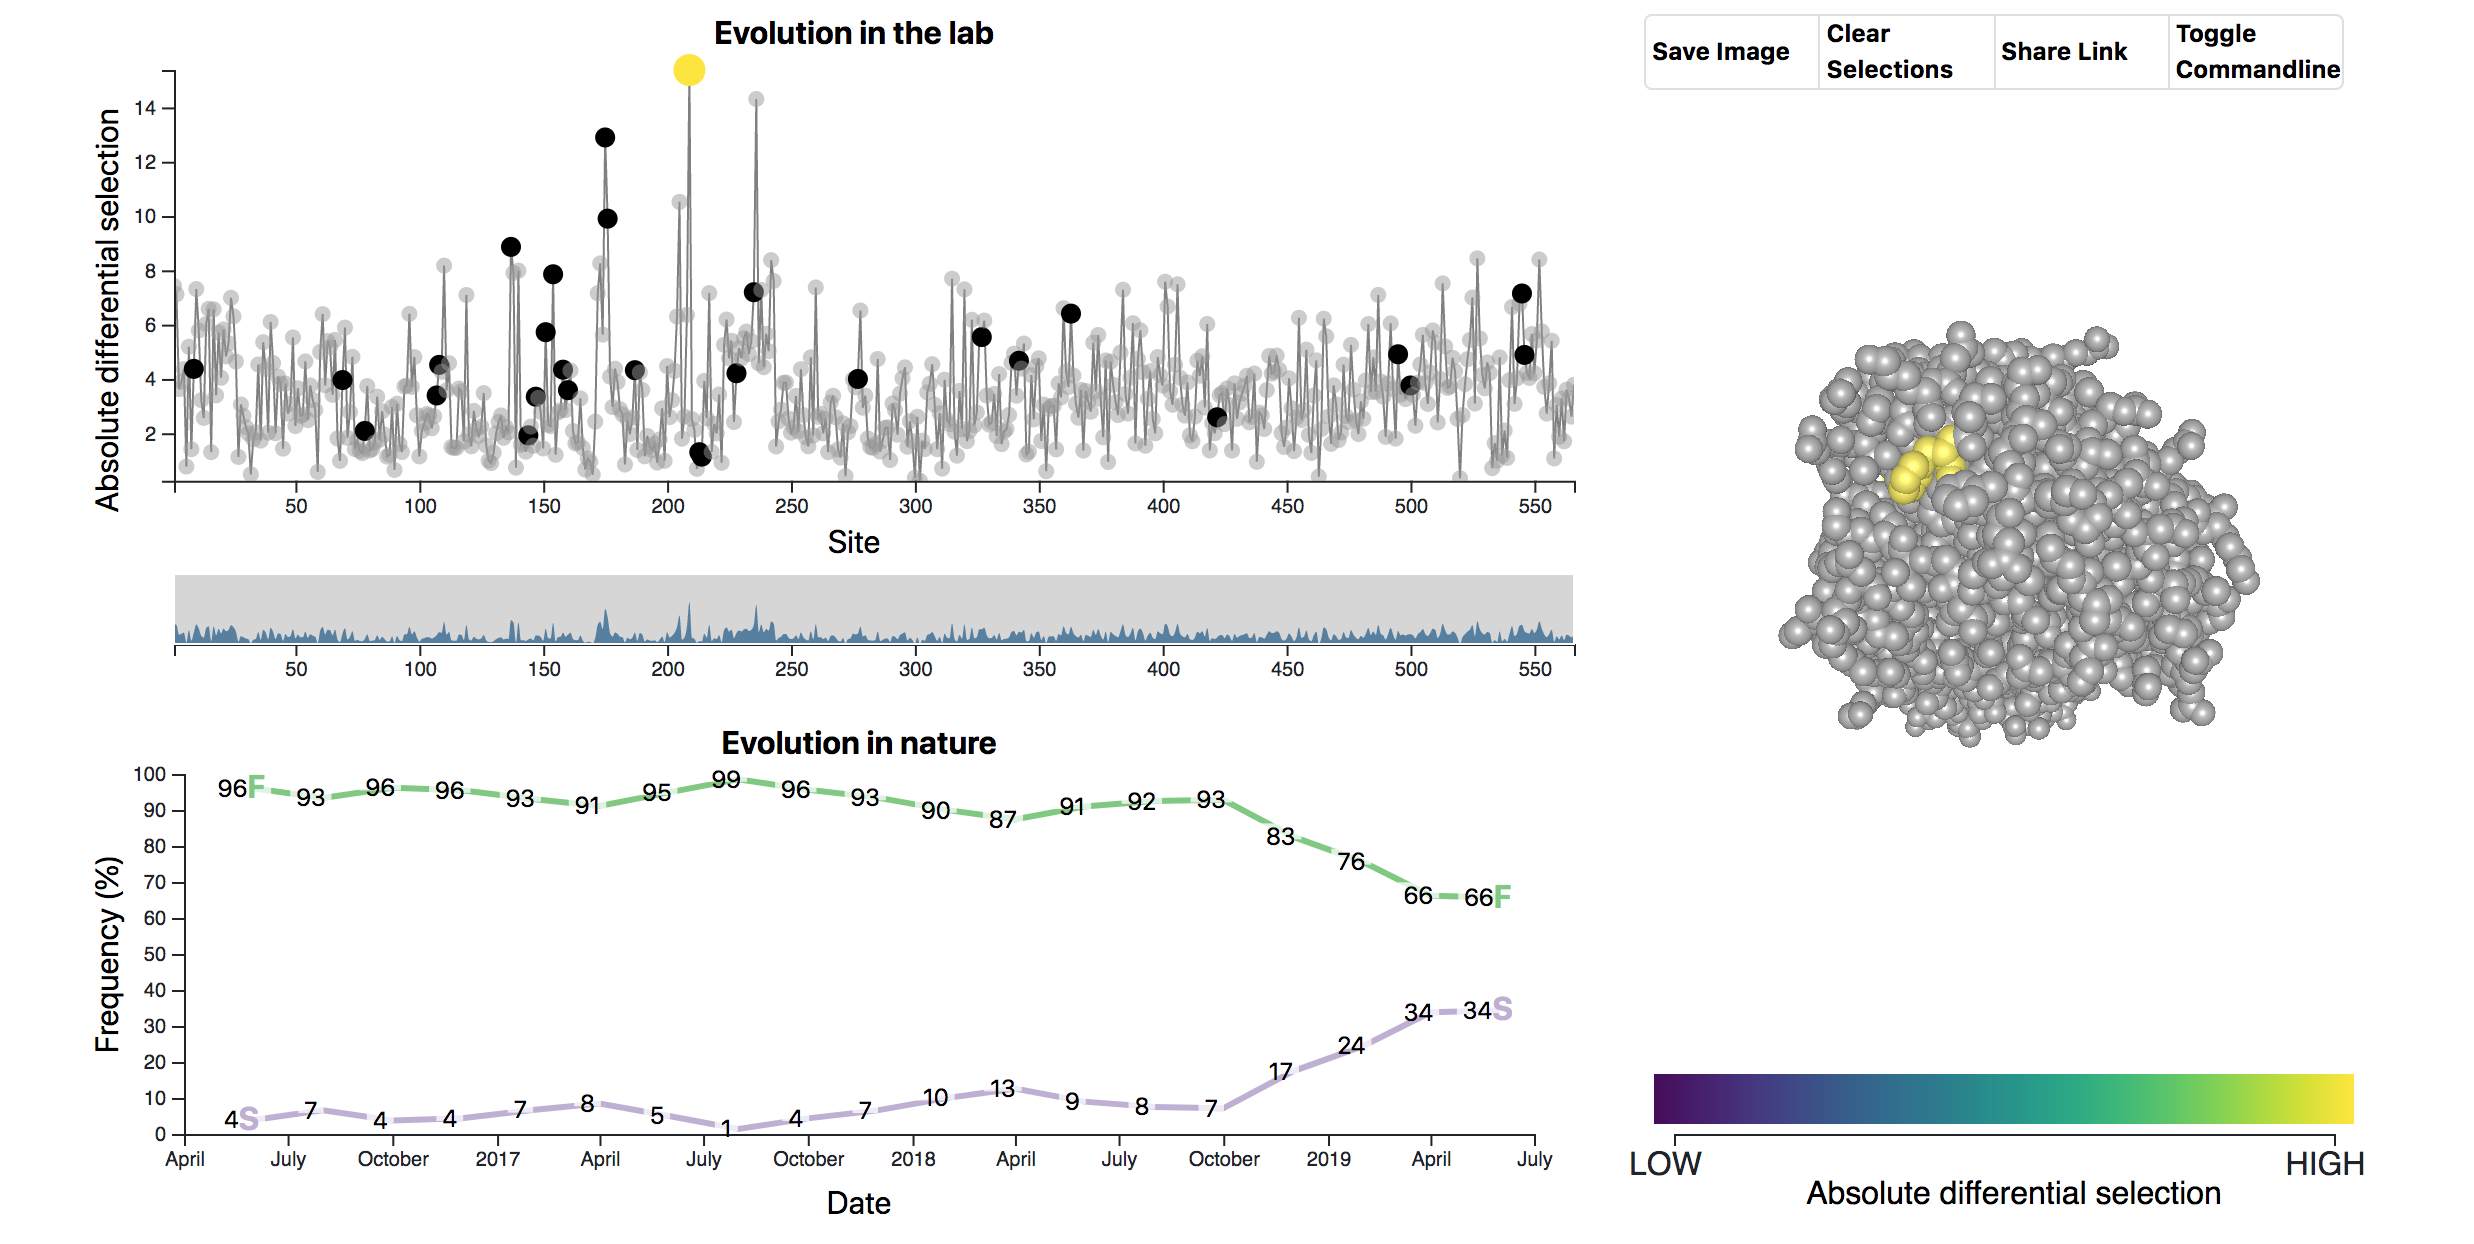
\includegraphics[width=1.0\textwidth]{viz-overview.png}
	\caption{\textbf{Full view of visualization platform.}
   The initial view of the visualization shows three panels: the laboratory-based DMS data, influenza variant frequencies in nature, and the 3D protein structure.
	}
	\label{overview}
\end{figure}

\subsection{DMS differential selection preferences}
Navigation of our visualization begins with the user selecting a site in the gene that they would like to explore.
Because the gene segments can be long, and many measurements are highly similar, it would be challenging to observe all measurements at once and interact with them.
To address this challenge, we have two plots within this data stream's panel, one that gives context about the overall positioning in the gene segment, and one that is the zoomed view that can be interacted with.
 To zoom in, the context panel can be brushed, and this will select the portion of the gene segment that the user would like to zoom in on.
Within the zoom panel, the DMS preferences by site, encoded using position, can be interacted with by mousing over the data points.
Mousing over brings up a tooltip providing additional details about the DMS data at that site.
In particular, the tooltip gives the exact value of the differential selection measurement, since this might be hard to read from looking at the y-axis.
The points can also be selected by clicking on them, which allows the user to enter the linked visualization, whereby the natural amino acid frequencies for that site, and that site in the 3D protein structure, will be selected.

\begin{figure}[H]
	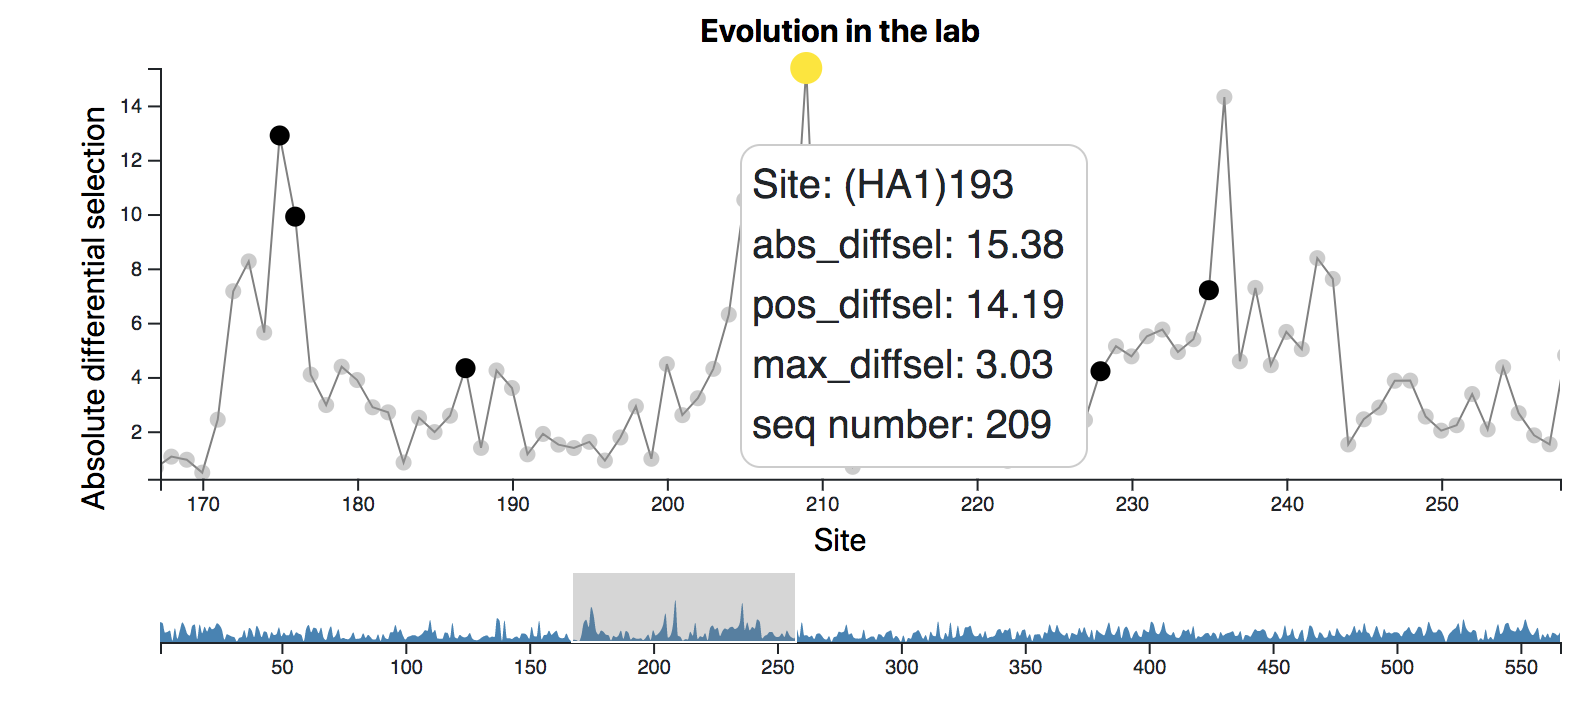
\includegraphics[width=1.0\textwidth]{dms-brushed-tooltip.png}
	\caption{\textbf{Visualization of differential selection data generated from DMS experiments.}
  The laboratory data can be explored and zoomed in on by brushing the context panel below the primary panel, giving both detail and overview to the user.
Sites that are colored black in this panel represent sites for which there is natural frequency data.
For all grey sites, only one variant of influenza at that site is found to circulate naturally.
Mousing over a tip brings up details on demand, and clicking on a data point selects that site for visualization in the other panels, and colors the point according to its maximal differential selection value.
	}
	\label{dms-data}
\end{figure}

\subsection{Amino acid frequencies observed in nature}
The natural amino acid frequencies are quantitative-ratio data that vary from 0 to 1 over time.
They are derived by asking, at different points in time, what proportion of all circulating influenza viruses have a specific amino acid at this site in the gene.
Given that these data are proportions, they take on values between 0 and 1, and data at cross-sectional time points sum to 1.
In our visualization, we have encoded these frequencies using position.
Selection of a site from the DMS preferences panel brings up a plotting space that shows which amino acids were observed at that position over time, and how those data changed through time.
We use position to encode the frequencies value, and color to differentiate between different amino acid residues.

\begin{figure}[H]
	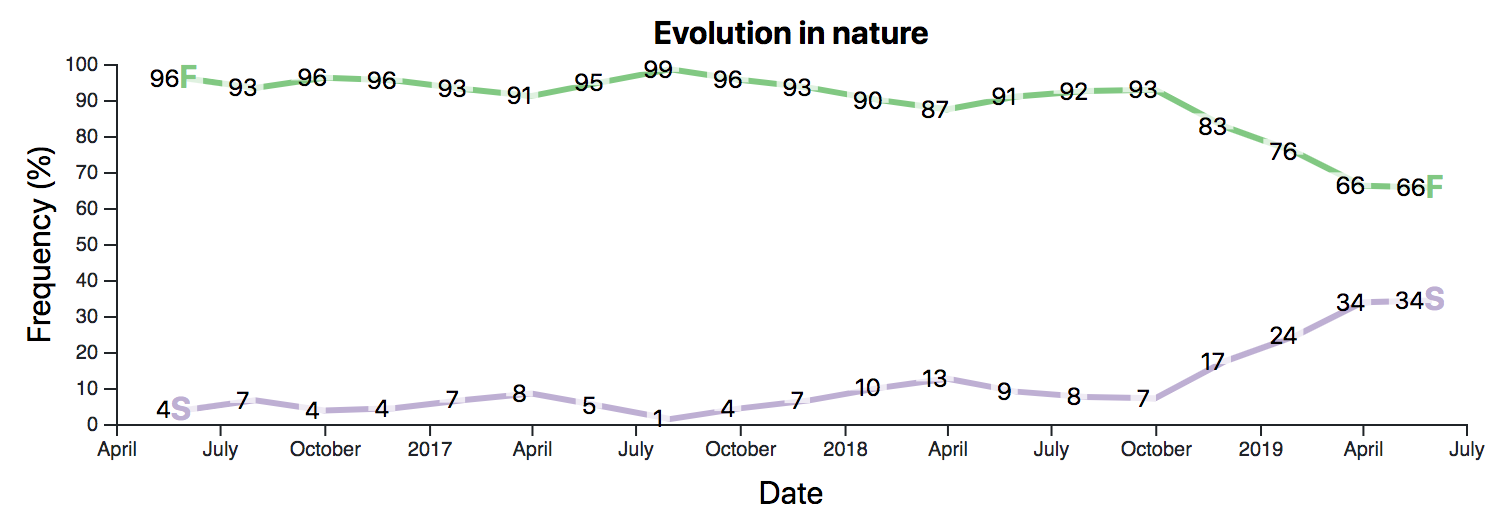
\includegraphics[width=1.0\textwidth]{frequencies-panel.png}
	\caption{\textbf{Frequencies of influenza variants in nature.}
  Once a site has been selected from the laboratory data panel, this panel shows the frequencies of influenza viruses with different amino acids at that site over the last three years.
In this example, at site 193 we see that there are two variants circulating, one has a phenylalanine (F) at this site, while the other has a serine (S).
We can see that the phenyalanine variant is at higher frequencies, but that the serine variant is rising in frequency.
  }
	\label{frequencies-panel}
\end{figure}

\subsection{3D protein structure}
Here, a selected site is differentiated from unselected sites by color.
All unselected sites are uniformly grey, and the selected site is colored.
The highlight color of the selected site is chosen according to the differential selection value of that site observed in the DMS data.

\begin{figure}[H]
	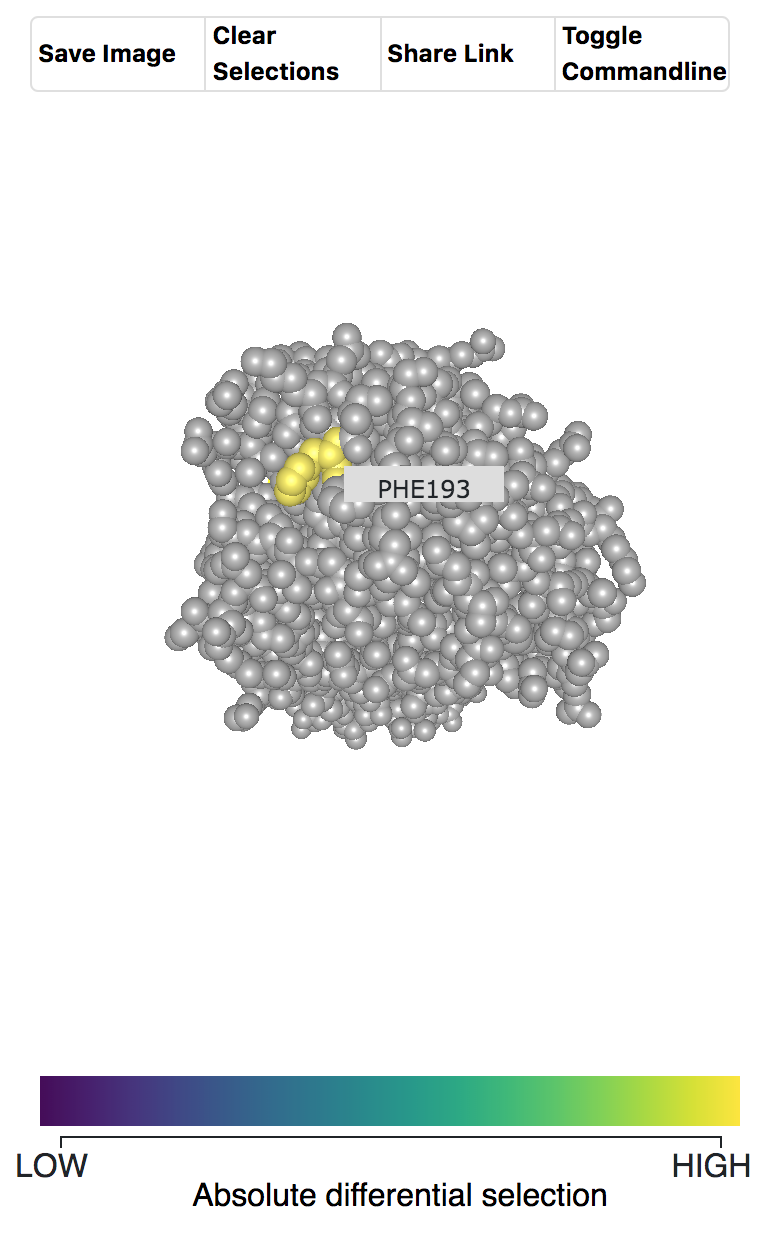
\includegraphics[width=1.0\textwidth]{3d-structure-panel.png}
	\caption{\textbf{3D protein structure with selected site highlighted.}
  3D protein structure panel, with the selected site colored according to its differential selection value.
The tooltip also provides information about which amino acid is at highest frequency at the site.
In this image, site 193 has a PHE, or phenylalanine.
  }
	\label{3d-structure}
\end{figure}

\section{Results}

The intended users of this visualization platform are researchers from a wide-range of disciplines.
These include clinicians and statisticians evaluating viral escape and the efficacy of immunotherapies in clinical trials, vaccinologists designing and evaluating immunogens and vaccines, evolutionary biologists studying viral evolution and immune evasion, and structural biologists interpreting the biological significance protein structures.
By building a platform that unifies relevant pieces of data, such as DMS preference data, naturally-occurring amino acid preferences, and protein structure information, the platform enables researchers to explore the interplay between viral evolution and antibody immunity, contextualize experimental data, and quickly address preliminary hypothesis with the data.
Most importantly, this type of data unification and presentation usually poses significant data curation and computational hurdles that non-computational biologists may struggle to perform.
The platform developed here lowers the bar necessary to explore the data, making access to these data, and the inferences that can be made from them, more broad.

\section{Discussion}

We created a browser-based visualization tool that allows the user to explore data generated from DMS experiments on influenza HA gene within the context of the 3D protein structure and of patterns of amino acid preferences observed in nature.
This platform, to our knowledge, provides the first such unified and interactive visualization of these data.
This unification helps to provides new insights to DMS preference data.
Firstly, hotspots of mutational tolerance or immune selection may not be easily intuited from the linear sequence data, since sites that are close to each other in the 3D protein may be quite distal in the sequence space.
Thus, tying these two views together improves the ease with which researchers can see whether changes at specific locations on the protein are responsible for immune escape and protein function.
Additionally, given the controlled environment of the lab, some researchers wonder to what extent DMS data recapitulates the evolutionary pathways observed in nature.
Our platform allows users to ask that exact question, by looking at both the frequencies of multiple amino acids observed at a site (that sites mutational tolerance in the lab and in nature), and also which amino acids specifically are observed (is the preferred amino acid in nature the same as the preferred amino acid in the lab).
Taken together, the ability to make new inferences across these data streams improves our ability to assess, analyze, and contextualize DMS studies.

\section{Future Work}

DMS experiments are conducted for various different genes, different pathogens, and outside of the field of infectious disease research as well.
As such, in the future we would like to expand this visualization platform to accept data sets other than from influenza.
To facilitate wider use, we would like to build functionality into the visualization platform such that it can take in drag-and-drop files for other protein structures and preferences.
Additionally, we would like to expand the number of panels that would allow joint visualization, for instance, by including phylogenetic trees that would allow querying of specific viruses with linking to relevant information about the virus and its proteins to relevant DMS data.

%%
%% The next two lines define the bibliography style to be used, and
%% the bibliography file.
\bibliographystyle{ACM-Reference-Format}
\bibliography{paper}

\end{document}
\endinput
%%
%% End of file.
